\PassOptionsToPackage{unicode}{hyperref}
\PassOptionsToPackage{hyphens}{url}
%
\documentclass[12pt, a4paper]{article}
\usepackage[a4paper,margin=1in]{geometry}
\setlength\parindent{0pt}
\usepackage{mathptmx}
\usepackage{amsmath,amssymb}
\usepackage[T1]{fontenc}
\usepackage[utf8]{inputenc}
\usepackage{textcomp}
\usepackage{comment}
\usepackage{hyperref}
\usepackage{graphicx}
\usepackage{float}
\usepackage{booktabs}
\usepackage{caption}

\author{Fabio Zanotti, Artificial Intelligence, ID number (matricola)
\\Edoardo Conca,  Artificial Intelligence ID number (matricola)
\\Antonio Morelli, Artificial Intelligence, ID number (matricola)}
\date{}
\title{International Trade Network Analysis: Understanding Global Economic Interactions}

\begin{document}
\maketitle

\section{Introduction}
\label{introduction}

International trade forms the backbone of the global economy, facilitating the exchange of goods, services, and resources between countries. The intricate web of trade relationships impacts not only national economies but also global economic stability and growth. Understanding these relationships is crucial for policymakers, economists, and business leaders alike. In this context, network analysis provides a powerful tool to unravel the complexities of international trade.

This study is situated within the field of economics, with a specific focus on international trade. By examining trade relationships between countries, we can uncover patterns, trends, and key players that shape global trade dynamics. Centrality measures are particularly useful in identifying countries that play a pivotal role in the trade network. These central countries often act as major hubs, significantly influencing trade flows and economic policies.

The main contributions of this project include the identification of central countries in the trade network using centrality measures, and the visualization of trade relationships and patterns through network graphs. Additionally, the analysis of the impact of key players on global trade flows provides further insights into the intricate dynamics of international trade.Through this approach, the study aims to provide valuable insights into the structure and behavior of international trade networks, thereby offering critical information for decision-makers in shaping economic strategies and policies.

\section{Problem and Motivation}
\label{problem-and-motivation}
One specific problem that this network analysis can potentially address is the identification of vulnerabilities within the global trade network. As global trade becomes increasingly interconnected, certain countries or trade routes may emerge as critical nodes or links. If these critical points were to be disrupted, whether by geopolitical conflicts, natural disasters, or economic sanctions, the impact on global trade could be significant. By identifying these vulnerabilities, policymakers and business leaders can develop strategies to mitigate risks, ensuring more resilient and stable trade networks. This could involve diversifying trade routes, establishing alternative partnerships, or investing in infrastructure improvements to enhance the robustness of the global trade system.

Therefore, the primary problem addressed in this study is the complexity of international trade networks and the challenge of identifying key patterns and influential players. Understanding these dynamics is crucial for several reasons:
\begin{itemize}
    \item Impact on National Economies: Central countries in the trade network significantly influence trade flows and economic policies.
    \item Global Economic Stability: Insights into trade networks help predict and mitigate economic instability.
    \item Policy Making: Data-driven analysis aids in formulating effective economic policies.
\end{itemize}

\subsection{Why International Trade?}
We believe international trade is essential for various reasons, particularly due to its significant impact on power dynamics, diplomacy, alliances, conflict, and cooperation. Trade relationships can shift power dynamics between nations, as countries with strong trade ties often wield more influence in international politics and negotiations. Moreover, trade agreements can lead to stronger diplomatic relations and strategic alliances, which in turn impact global peace and security. Economic interdependence through trade can both mitigate and exacerbate conflicts; while trade promotes cooperation and mutual benefits, it can also become a point of contention, influencing geopolitical stability. 

Understanding international trade through network analysis offers several valuable insights, especially for students, young professionals, and the new generation. Knowledge of global trade dynamics is crucial for careers in economics, business, international relations, and public policy. Being aware of how trade impacts economies and geopolitics helps in making informed decisions as future leaders and policymakers. Analyzing trade networks fosters a deeper understanding of global interconnectedness and the importance of international cooperation. \\This study aims to provide valuable insights into the structure and behavior of international trade networks, offering critical information for decision-makers in shaping economic strategies and policies. By understanding the central players and patterns within the trade network, we can better anticipate and respond to global economic and political challenges, ultimately contributing to a more stable and prosperous world.

\begin{comment}
\subsection{Why International Trade?}
There are several reasons on why we chose International trade as main topic of our analysis. We think IT results essential for three reasons in particular:
\begin{itemize}
    \item **Power Dynamics**: Trade relationships can shift power dynamics between nations. Countries with strong trade ties often have more influence in international politics and negotiations.
    \item **Diplomacy and Alliances**: Trade agreements can lead to stronger diplomatic relations and strategic alliances, impacting global peace and security.
    \item **Conflict and Cooperation**: Economic interdependence through trade can both mitigate and exacerbate conflicts. While trade can promote cooperation and mutual benefits, it can also become a point of contention, influencing geopolitical stability.
    \item Consumer Benefits: It provides consumers with a broader range of products and services, often at lower prices, enhancing their quality of life.
\end{itemize}
Moreover, we think that understanding international trade through network analysis provides several valuable insights, expecially in these days, for students, young professionals, and the new generation about:
\begin{itemize}
    \item **Career Opportunities**: Knowledge of global trade dynamics is crucial for careers in economics, business, international relations, and public policy.
    \item Informed Decision-Making: Awareness of how trade impacts economies and geopolitics helps in making informed decisions as future leaders and policymakers.
    \item Global Awareness: Analyzing trade networks fosters a deeper understanding of global interconnectedness and the importance of international cooperation.
    \item Innovative Thinking: Exposure to complex systems and analytical tools like network analysis encourages innovative thinking and problem-solving skills.
\end{itemize}

In conclusion, through this approach, the study aims to provide valuable insights into the structure and behavior of international trade networks, offering critical information for decision-makers in shaping economic strategies and policies. By understanding the central players and patterns within the trade network, we can better anticipate and respond to global economic and political challenges, ultimately contributing to a more stable and prosperous world.
\end{comment}

\section{Datasets}
\label{datasets}
The \href{https://www.kaggle.com/datasets/lucafrance/the-world-factbook-by-cia}{World Factbook} dataset provides basic intelligence on the history, people, government, economy, energy, geography, environment, communications, transportation, military, terrorism, and transnational issues for 265 world entities collected by the CIA (Central Intelligence Agency). The data for this project was gathered from the JSON file \textit{countries.json}, which includes information about various countries involved in international trade. This data was then processed and converted into pandas DataFrames using Python libraries such as json, networkx, and plotly.

The dataset contained a multitude of attributes, which were first filtered and mapped to more manageable names for ease of analysis. Key economic indicators such as GDP, export and import values, and trade partners were selected and renamed using a predefined mapping. Only countries that contained all the relevant attributes were retained for further analysis.

Subsequently, the data underwent a cleaning process to remove unwanted characters, ensuring that the values were in a usable format. Trade partners for both exports and imports were extracted from their respective strings and converted into dictionaries with the partners as keys and their corresponding trade percentages as values.
\\
\\Two primary DataFrames were created: one for exports and one for imports. Each DataFrame represents respectively the exports and imports trades relationships between countries, with columns indicating the source country, target country, and the weight of the trade relationship (percentage of trade).

\begin{figure}[ht]
\centering
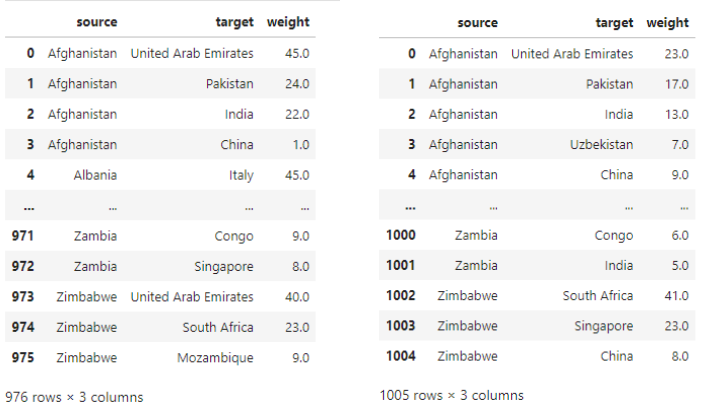
\includegraphics[scale=0.4]{img/import_export.drawio.png}
\captionsetup{font=scriptsize,labelfont=bf}
\caption{Import and Export DataFrames}
\label{fig:dataframes}
\end{figure}

Using these DataFrames and the NetworkX library, two directed networks were constructed for both exports and imports. We decided to keep the two related aspects of international trade separate, in order to obtain more specific insights and draw comparisons between them. To facilitate the superimposition of the structures and results, we proceeded to remove 2 nodes from the exports network ('\emph{Guadeloupe}', '\emph{Martinique}'), since they weren't present in the import network and they had just one edge each in the exports network, placing them in a peripheral position in the graph. 
\begin{table}[h]
\centering
\small
\scalebox{0.8}{%
\begin{tabular}{lllll}
\toprule
& \multicolumn{2}{c}{Before Cleaning} & \multicolumn{2}{c}{After Cleaning} \\
\cmidrule(lr){2-3} \cmidrule(lr){4-5}
& Exports & Imports & Exports & Imports \\
\midrule
Nodes & 209 & 207  & 207 & 207   \\
Edges & 974 & 1003 & 972 & 1003  \\
\bottomrule
\end{tabular}
}
\captionsetup{font=scriptsize,labelfont=bf}
\caption{Comparison of Network Statistics before and after cleaning}
\label{tab:network_stats}
\end{table}

Together with NetworkX itself, we used the Plotly library to facilitate the visualization of the networks, making them interactive and zoomable. Figs. \label{fig:exportsnet} and \ref{fig:importsnet} show a static render obtained respectively from the exports and imports network.
\begin{figure}[ht]
\centering
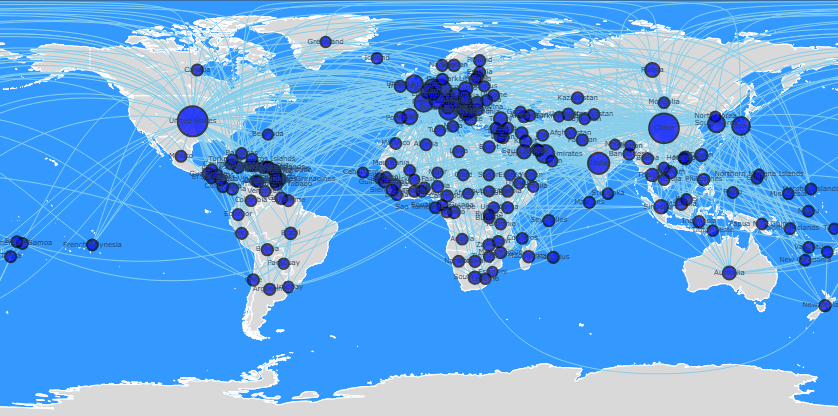
\includegraphics[scale=0.6]{img/exportnet.png}
\captionsetup{font=scriptsize,labelfont=bf}
\caption{Exports Network render, node size coded by degree centrality}
\label{fig:exportsnet}
\end{figure}

\begin{comment}
For instance, centrality measures were applied to uncover key players in the trade network, revealing which countries acted as major hubs influencing trade flows and economic policies.

Visualizations of these networks were created to better understand the different roles countries play in global trade. By analyzing the separate networks for imports and exports, it was possible to discern countries that were central in one network but peripheral in another. This dual analysis provided a comprehensive view of the trade dynamics.

In conclusion, the analysis culminated in the creation of network graphs that visually represented the trade relationships and patterns among countries. This approach not only highlighted the central countries in the trade network but also illustrated the impact of key players on global trade flows. The final result was two DataFrames, one for exports and one for imports, each detailing the intricate web of international trade relationships.
\end{comment}



\section{Validity and Reliability}
\label{validity-and-reliability-not-needed-for-the-project-proposal}

The model's validity is assessed by how accurately it represents the actual international trade relationships. This involves ensuring that the dataset accurately reflects real-world trade data and that the network analysis methods used are appropriate for this type of data. Therefore, in assessing the validity of our study, we consider how closely the model and analysis represent the reality of international trade dynamics. The \textit{World Factbook} dataset from the CIA provides a comprehensive overview of countries' economic indicators, which serves as a foundational source for our analysis. By utilizing this dataset, we aim to capture a broad spectrum of factors that influence trade relationships, such as GDP, export-import ratios, and trade partner networks. However, it's important to note that while these indicators are robust, they are subject to limitations inherent in any dataset, such as potential inaccuracies in reporting or timeliness.
\\
\\Regarding reliability, our approach involves transforming raw data into structured formats suitable for network analysis using, as before mentioned, Python libraries like pandas and networkx. The cleaning and preprocessing steps ensure consistency and accuracy in our findings, minimizing errors that could arise from data formatting discrepancies. By documenting our methodology and providing transparency in data handling, we aim to enhance the reproducibility of our study. This allows for future researchers to replicate our analysis, validate our conclusions, and build upon our findings in the field of international trade network analysis.
\\Overall, it's important to notice that, while our study leverages robust datasets and rigorous analytical methods to uncover insights into global trade dynamics, the validity depends on the accuracy and completeness of the underlying data sources. Our commitment to transparency and methodological rigor supports the reliability of our findings, facilitating reproducibility and further exploration in this area.
\begin{figure}[ht]
\centering
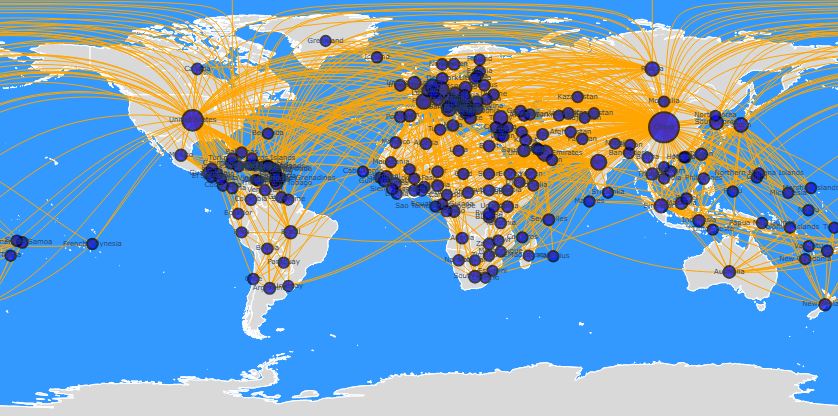
\includegraphics[scale=0.6]{img/importsnet.png}
\captionsetup{font=scriptsize,labelfont=bf}
\caption{Imports Network render, node size coded by degree centrality}
\label{fig:importsnet}
\end{figure}
\section{Measures and Results}
\label{measures}
\subsection{Measures}

The following measures were applied:
\begin{itemize}
\item \textbf{Node Metrics}:
\begin{itemize}
    \item \textbf{Degree Centrality}: indicates the number of trade partners a country has. A higher degree centrality means that a country has more direct trade relationships.
    \item \textbf{Eigenvector Centrality}: identifies countries that are not only well-connected but are connected to other highly influential countries.  Measures a country's influence based on the quality of its connections.
    \item \textbf{Betweenness Centrality}: indicates the countries that act as intermediaries in trade routes, controlling the flow of goods between other nations. A country with high betweenness centrality has significant influence over trade flow and can impact the efficiency of global trade routes.
    \item \textbf{Closeness centrality}: indicates how efficiently a country can access other countries' markets. A higher closeness centrality suggests that a country is geographically or economically well-positioned to trade with others, reducing trade costs and improving market access.
    \item \textbf{Pagerank}: indicates the overall importance of a country within the global trade network. A high PageRank score suggests that a country is a significant hub, attracting substantial trade from other countries.
    \item \textbf{Local Clustering Coefficient}: indicates the extent to which countries tend to form trade blocs or regional trade agreements. A higher clustering coefficient suggests that countries tend to trade more with their neighbors, forming tightly-knit clusters.
\end{itemize}
\item \textbf{Network Metrics}:
\begin{itemize}
    \item \textbf{Centrality Distributions - Centrality Cumulative Distributions}: crucial for understanding the connectivity pattern within a trade network. Fitting this distribution to a power law can reveal whether the network has a scale-free structure, characterized by a few highly connected nodes (hubs) and many nodes with fewer connections. This is significant because it indicates the presence of dominant countries that act as major trade hubs, which can have substantial implications for network resilience, trade flow efficiency, and economic influence.
        \item \textbf{Correlation between Local Clustering Coefficient and Degree Centrality}: by correlating Degree Centrality (DC) and Local Clustering Coefficient (LCC) in trade networks, we reveal how countries with more trade connections (higher DC) tend to have trading partners that are themselves well-connected (higher LCC), influencing network structure and trade dynamics.
     \item \textbf{Cliques}: refer to tightly-knit groups of countries that extensively trade among themselves. These cliques can represent regional trade blocs or economic alliances where countries within the clique have strong and frequent trade interactions.
     \item \textbf{K-core Decomposition}: we can identify the most influential and interconnected nodes within the trade network. These core nodes are crucial for understanding the backbone and the periphery of the trade network, as they often represent countries with strong and diverse trade relationships.
    \item \textbf{Assortative Mixing by Degree}:  indicates whether countries with similar trade volumes tend to trade with each other. High assortative mixing suggests that countries with high trade volumes (high-degree nodes) tend to trade more with other high-volume countries, while low assortative mixing might indicate a more diverse set of trade partners irrespective of trade volume.
    \item \textbf{Density}:  indicates the overall connectivity among countries. A denser network suggests that there are more trade relationships between countries, indicating a more interconnected and potentially robust global trade system.

\end{itemize}
\end{itemize}
The application of these measures allows for a comprehensive analysis of the global trade network, shedding light on the roles and influence of different countries. By examining node metrics, we can understand individual country significance, while network metrics provide insights into the overall structure and connectivity of international trade. This dual approach helps identify key trade hubs, regional trade blocs, and the interdependencies within the global trade system, ultimately contributing to more informed economic policies and strategies.
\subsection{Results}
\subsubsection{Degree Centrality}
\begin{figure}[ht]
\centering
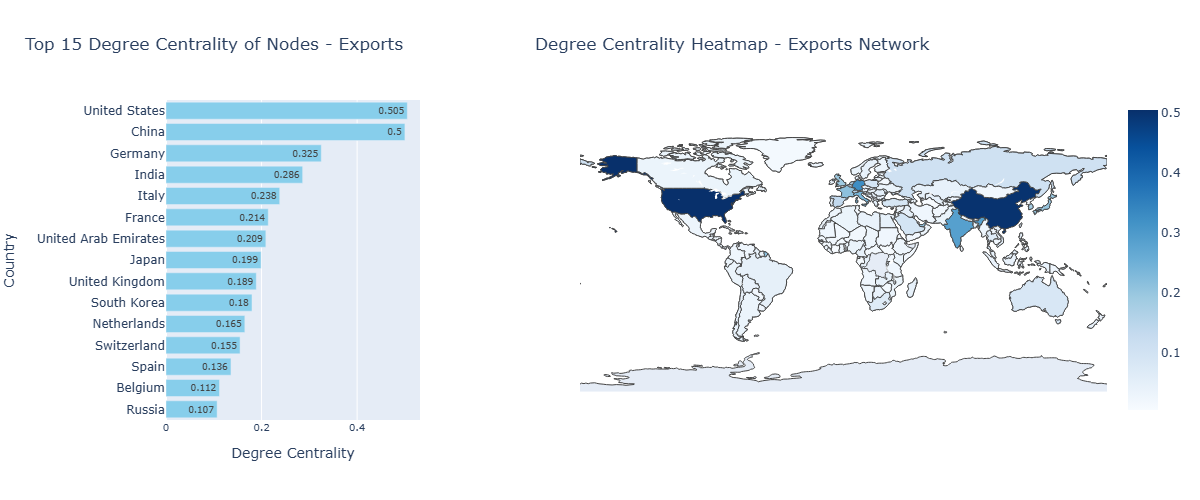
\includegraphics[width=\textwidth]{img/exportdegree.png}
\label{fig:exportdegree}
\end{figure}
The United States and China are important participants in the global export network, as indicated by their high degree centrality values (0.5049 and 0.5000). They are significant in international trade because of their direct commercial ties to numerous nations. Germany and France exhibit noteworthy degree centrality values (0.3252 and 0.2136), which are indicative of their robust export connections both domestically and internationally.
India's degree centrality of 0.2864 indicates that it is becoming more and more important in global commerce. Its varied export base and growing economy could be the cause of this.
\begin{figure}[ht]
\centering
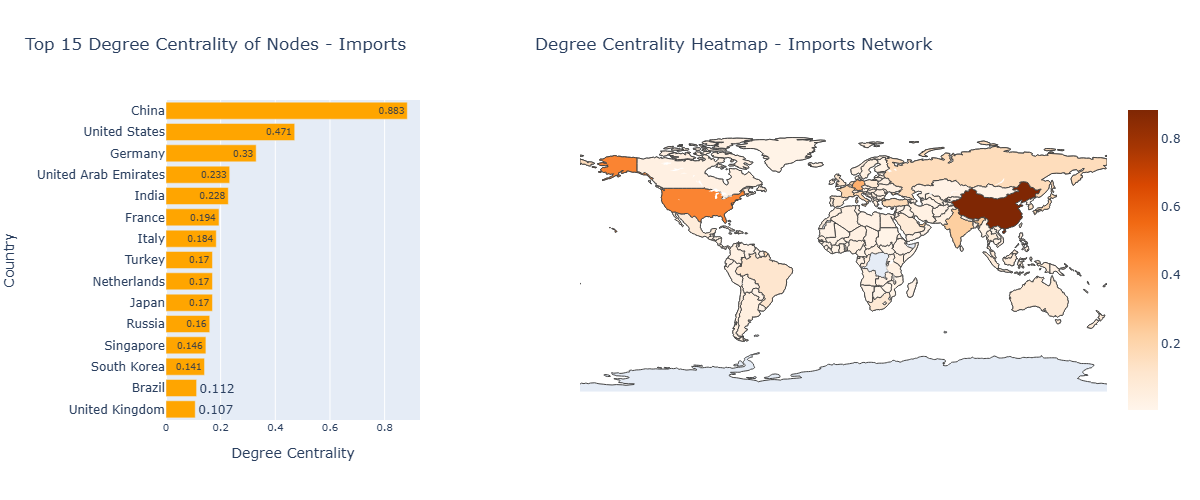
\includegraphics[width=\textwidth]{img/importdegree.png}
\label{fig:importdegree}
\end{figure}
\\China is the most linked nation in the import network, with a degree centrality of 0.8835, which reflects the enormous demand it has for imports to support its production and consumption.
United States, driven by its sizable consumer market and diverse economy, has high degree centrality (0.4709) which denotes its essential role as a major importer.
Germany also plays an important position in the European and international supply chains, as evidenced by its degree centrality (0.3301) in imports, which is comparable to its export role.\\
The data reveals strong bilateral trade relations between major economies. For instance, the high centrality values of the United States and China in both export and import networks suggest robust trade ties.
As seen by their high degree centrality scores, nations like Germany, China, and the US are important hubs for global commerce. The degree of integration of their economies into the global trade system has an impact on trade flows worldwide.
India and the United Arab Emirates exhibit significant centrality values, demonstrating their increasing clout and incorporation into international commerce networks.
Regional Trade Patterns  are further highlighted by the degree centrality values. While North America, led by the United States, exhibits tremendous connectedness, Europe and Asia have dense trading networks.\\
\paragraph{Degree Centrality Distributions}
\begin{figure}[ht]
\centering
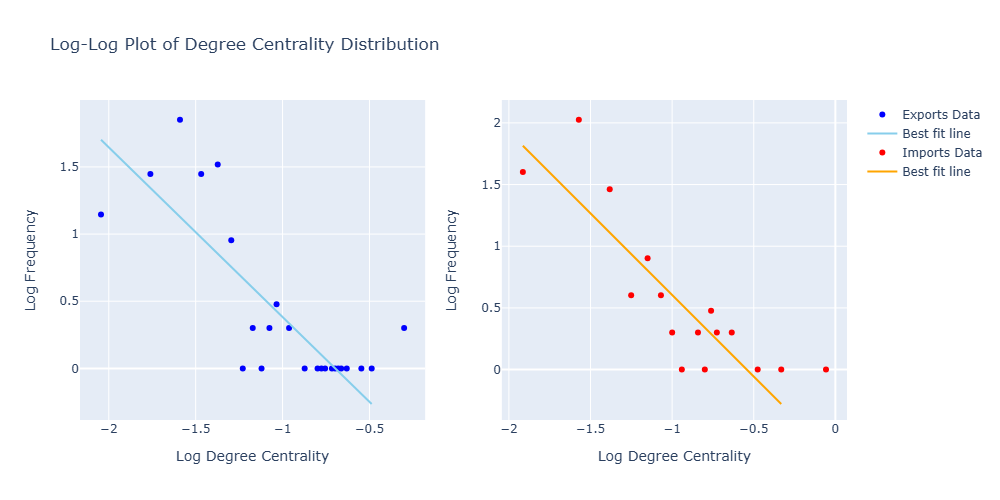
\includegraphics[scale=0.4]{img/degreedist.png}
\label{fig:degreedist}
\end{figure}
The negative slope values (-1.263 for exports and -1.323 for imports) indicate that as the degree centrality increases, the frequency of nodes with that centrality decreases. This is consistent with a power-law distribution, suggesting the presence of a few highly connected hubs and many nodes with fewer connections.

The very low p-values (8.1e-5 for exports and 2.6e-5 for imports) indicate that the observed relationship between the degree centrality and its frequency is statistically significant. This strengthens the evidence that the degree centrality follows a power-law distribution.

The high negative R-values (-0.83 for exports and -0.87 for imports) suggest a strong negative correlation between the log-transformed degree centrality and its frequency. This confirms the power-law behavior of the network, indicating that the trade network is likely to be scale-free.

The degree centrality distribution analysis reveals that both the export and import networks exhibit characteristics of scale-free networks. This means that a few countries (nodes) play a crucial role as major hubs in global trade, while many countries have fewer trade connections. Understanding this structure is vital for policy-making and economic strategies, as these hubs are critical for the stability and efficiency of the global trade network. Identifying and supporting these hubs can enhance global trade resilience and efficiency, while also highlighting potential vulnerabilities if these hubs were to be disrupted.
\begin{figure}[ht]
\centering
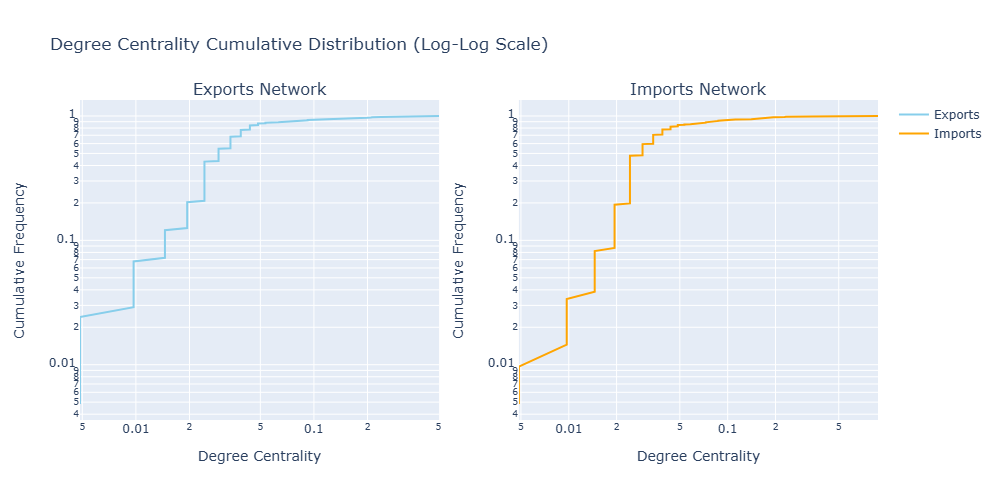
\includegraphics[scale=0.4]{img/degreecum.png}
\label{fig:degreedist}
\end{figure}
Observing the log-log plots we can have more details about the distribution's tail: it shows a more linear trend in the middle range, suggesting a potential power-law distribution, as previously highlighted.

The steep rise in the CDF at low degree centrality values, followed by a gradual increase, suggests heterogeneous network structures where a few countries are significantly more connected than others. The presence of highly connected countries (high degree centrality) implies that these countries act as major hubs in both the network. These hubs are crucial for the stability and efficiency of global trade.
\subsubsection{Eigenvector Centrality}
\begin{figure}[ht]
\centering
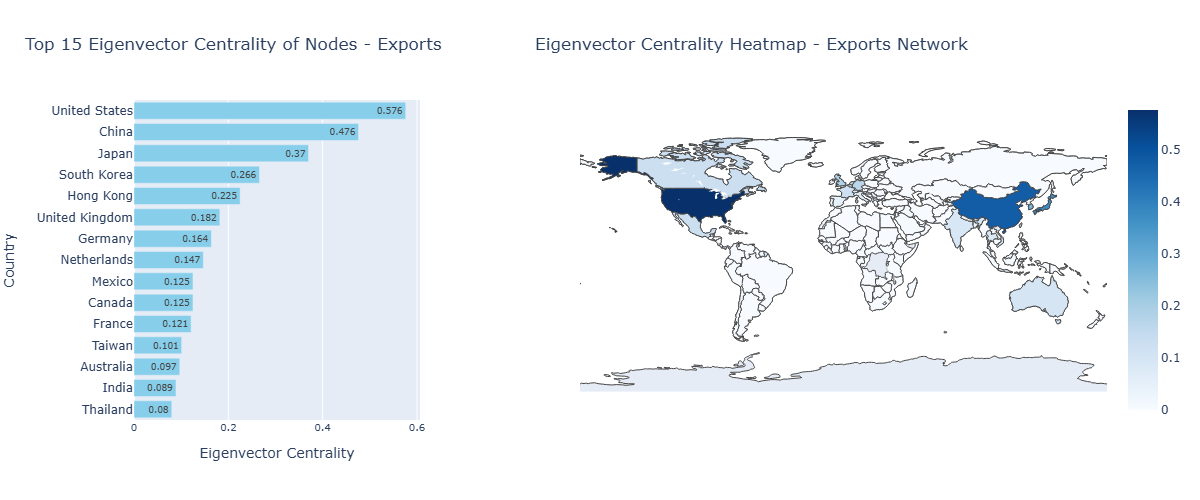
\includegraphics[width=\textwidth]{img/exporteigen.png}
\label{fig:exporteigen}
\end{figure}
The country with the highest eigenvector centrality, the United States (0.5758), is clearly in an influential position within the exports network. The US's central role is reinforced by its connections to other highly influential nodes. The rest of the highest centrality countries belongs to the eastern side of the world: China (0.4764), followed by Japan (0.3699), South Korea (0.2661) and Hong Kong (0.2246).
\begin{figure}[ht]
\centering
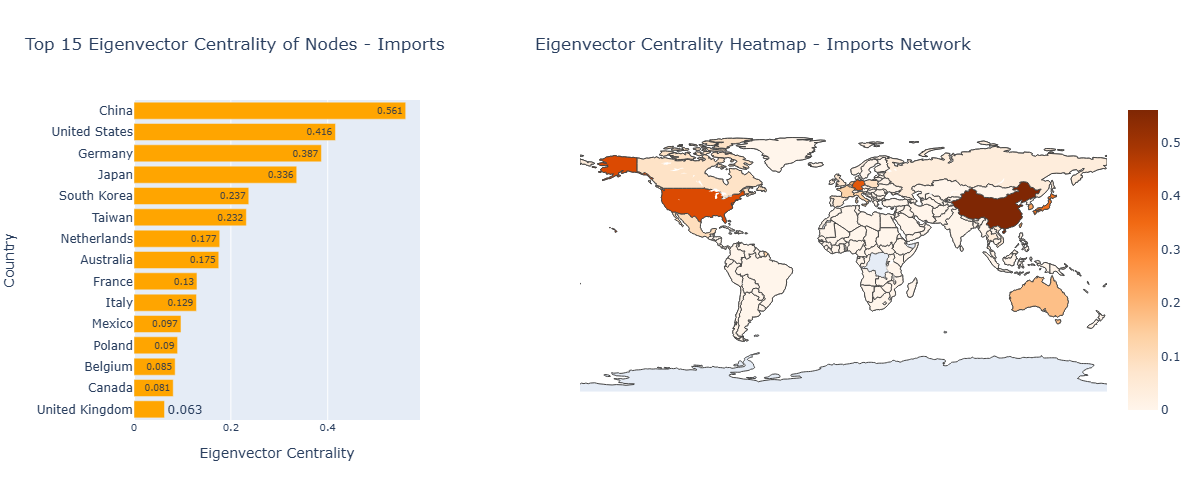
\includegraphics[width=\textwidth]{img/importeigen.png}
\label{fig:importeigen}
\end{figure}
By looking at the Eigenvector Centrality values of the Imports Network, we can immediately see that China (0.5607) and the United States (0.4158) swiched positions at the top, while still being the most two influential nodes. We notice a higher eigenvector centrality value in Germany (0.3870 in the imports network compared to 0.1636 in exports), demonstrating its higher influence.\\
The dominance of China and the United States in the export and import networks is indicative of their important roles in world trade. South Korea, Japan, and Germany are all heavily represented in both networks, demonstrating their significance.

Certain nations play distinct roles in both imports and exports. For instance, when it comes to imports, Canada and Mexico have greater influence. While they play a more significant role in exports, France and Italy have a moderate effect in both networks. Europe has a crucial role in international trade, as evidenced by the relative influence of European nations like the Netherlands, Germany, and the United Kingdom in both networks.

Numerous nations have 0 eigenvector centrality in both networks, suggesting their restricted involvement in international trade relations. These nations might trade less diversifiedly, have smaller economies, or be more regionally focused.
\paragraph{Eigenvector Centrality Distributions}
\begin{figure}[ht]
\centering
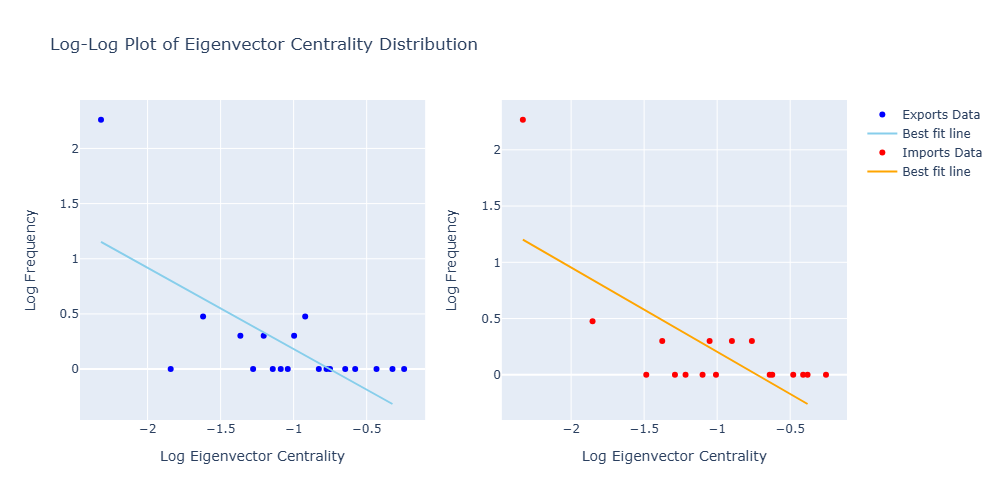
\includegraphics[scale=0.4]{img/eigendist.png}
\label{fig:eigendist}
\end{figure}
The slopes for both networks are negative, indicating a decreasing trend. In a power-law distribution, this suggests that high eigenvector centrality values are less frequent, while lower values are more common. The slopes are quite similar (-0.7364 for exports and -0.7493 for imports), indicating a similar rate of decay in the centrality distributions across both networks.

Both p-values (1.6e-03 for exports and 1.9e-03 for imports) are very low, indicating that the slope is statistically significant. This means the fit of the power-law model to the centrality data is robust.

The R-values (-0.69 for exports and -0.71 for imports) are negative and close to -0.7, indicating a moderate to strong negative correlation. This suggests that as the eigenvector centrality increases, the frequency of such nodes decreases, which is expected in networks where a few nodes have high centrality and many nodes have low centrality.

The analysis of the eigenvector centrality distributions for both the exports and imports networks demonstrates a typical power-law behavior. A few countries (nodes) dominate in terms of centrality, having significant influence and connections, while the majority have lower centrality values. This distribution is consistent with many real-world networks where influence or connectivity is not evenly distributed.
\begin{figure}[ht]
\centering
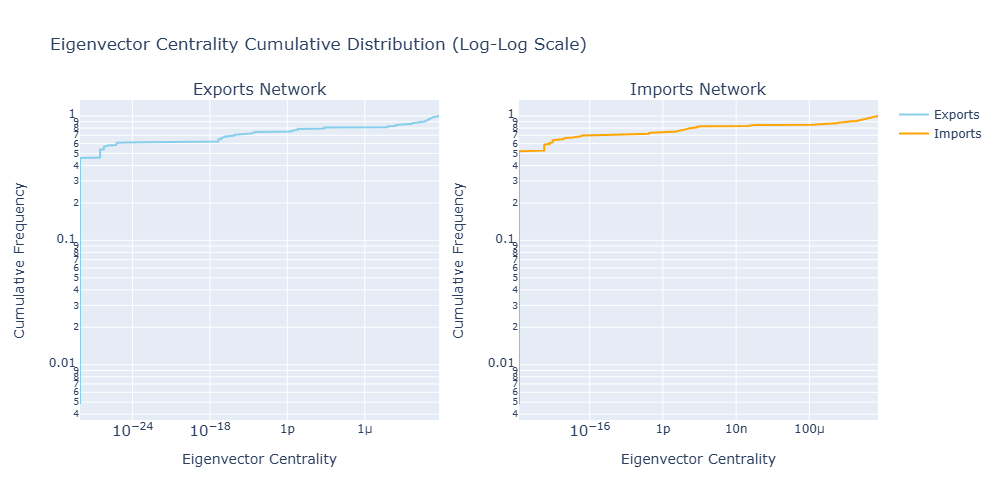
\includegraphics[scale=0.4]{img/eigencum.png}
\label{fig:eigencum}
\end{figure}
The CDF increases sharply at very low values of eigenvector centrality. This indicates that most nodes (countries) have low eigenvector centrality, suggesting they are not highly influential within the networks. These countries might depend on the central nodes for their connections and are less influential in shaping the overall network.

The log-log plots show a long tail, indicating the presence of a few countries with significantly higher eigenvector centrality. This suggests that small number of countries are highly central and influential within both networks.

The networks likely exhibits a hierarchical structure, typical of many natural and social networks, where a small number of nodes play a crucial role in maintaining the network's integrity.
\subsubsection{Betweenness Centrality}
\begin{figure}[ht]
\centering
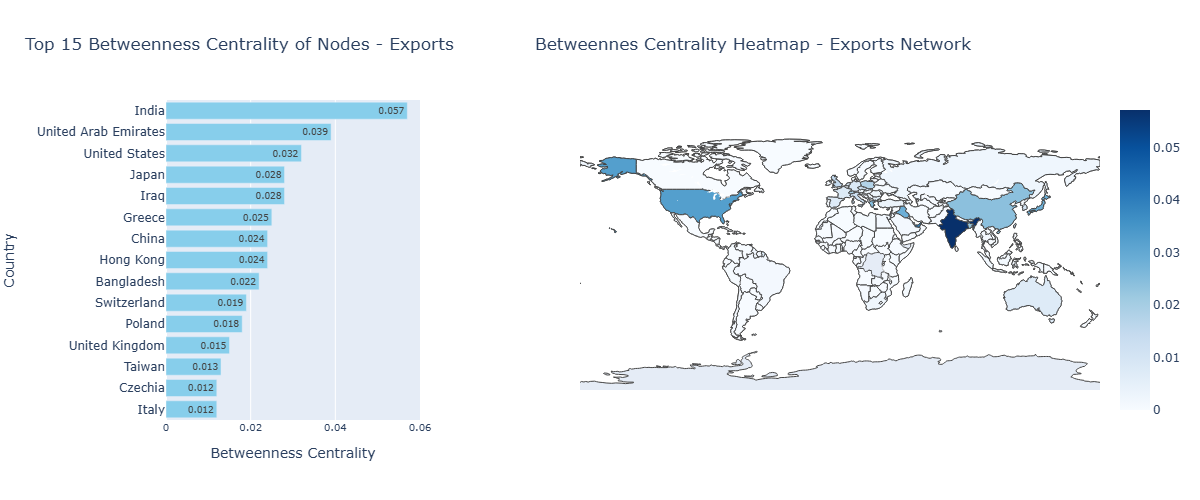
\includegraphics[width=\textwidth]{img/exportbetween.png}
\label{fig:exportbetween}
\end{figure}
With the highest betweenness centrality (0.0571) in the export network, India plays a crucial role in fostering economic relations with other nations. Important nodes in the network that serve as important hubs for commerce routes are the United States (0.0325) and the United Arab Emirates (0.0393). Japan (0.0284) and Iraq (0.0282) also play important roles as intermediaries. are essential to preserving the flow of commodities and have an impact on the network's stability and effectiveness.

Numerous nations have extremely low betweenness centrality scores, such as Botswana (0.0005), Antigua \& Barbuda (0.0004), and Albania (0.0001), indicating that they are peripheral nodes in the network with minimal intermediate trade linkages.\\

\begin{figure}[ht]
\centering
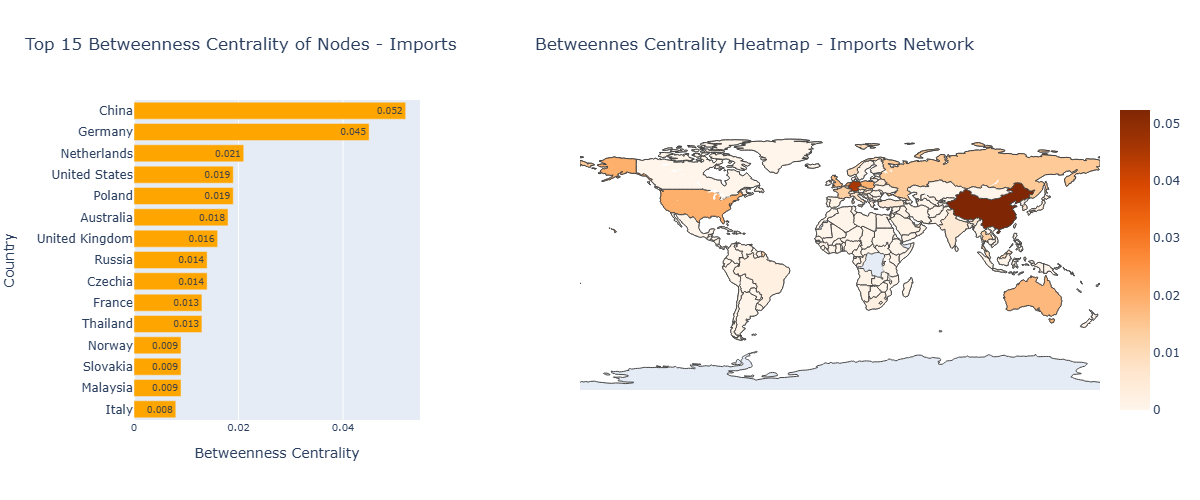
\includegraphics[width=\textwidth]{img/importbetween.png}
\label{fig:importbetween}
\end{figure}
China (0.0523) and Germany (0.0455) have the highest betweenness centrality in the import network, followed by a group of 4 countries: United States (0.0195), Poland (0.0192), Netherlands (0.0208), and United Kingdom (0.0164) which are also key intermediaries.

Many countries, such as Samoa (0.0000), Panama (0.0000), and Ukraine (0.0000), have zero betweenness centrality, indicating they are on the periphery of the import network.\\
Both networks emphasize certain nations—like the US, China, and Germany—as important hubs due of their substantial contributions to international trade, but show a large number of smaller or less strong nations as peripheral nodes, suggesting a limited impact on international trade flows.

There are variations in centrality levels between import and export networks in some countries. As an example, China is central in both networks but particularly dominating in imports, while India is highly key in the export network but less so in the import network.
\paragraph{Betweenness Centrality Distributions}
\begin{figure}[ht]
\centering
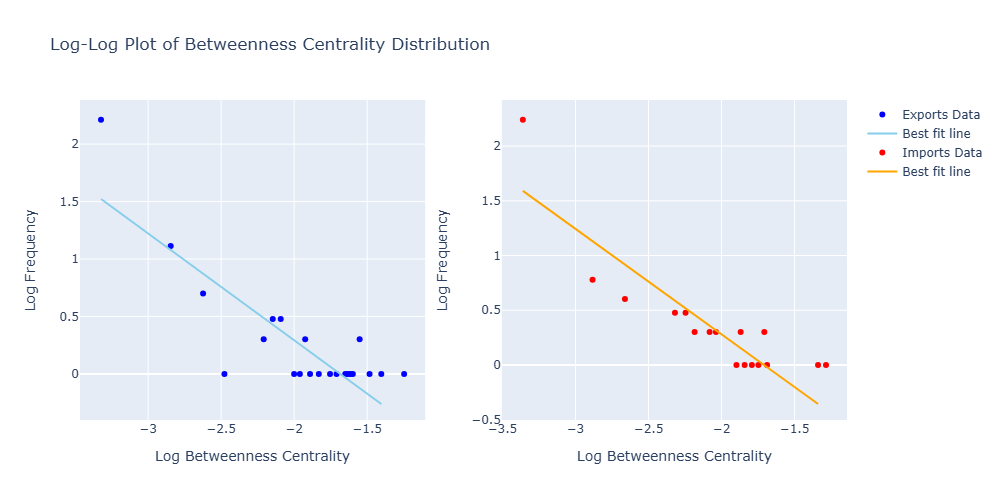
\includegraphics[scale=0.4]{img/betweendist.png}
\label{fig:betweendist}
\end{figure}
The negative slopes in the log-log plot suggest that betweenness centrality in both export and import networks follows a power-law distribution. This implies that a small number of countries have very high betweenness centrality, acting as major hubs or bridges in the network, while the majority of countries have low betweenness centrality.

The high absolute values of the R-values (-0.85 for exports and -0.89 for imports) indicate a strong linear relationship on the log-log scale, further confirming the power-law nature of the distribution.

The very low p-values (1.3e-06 for exports and 4.9e-06 for imports) suggest that the results are statistically significant. This means that the observed power-law distribution is not due to random chance and reflects a fundamental characteristic of the trade networks.

The reliance on a few key countries for maintaining the flow of goods highlights potential vulnerabilities. Disruptions in these central hubs can have a widespread impact on the entire network, emphasizing the need for robust trade policies and diversification of trade routes.
\begin{figure}[ht]
\centering
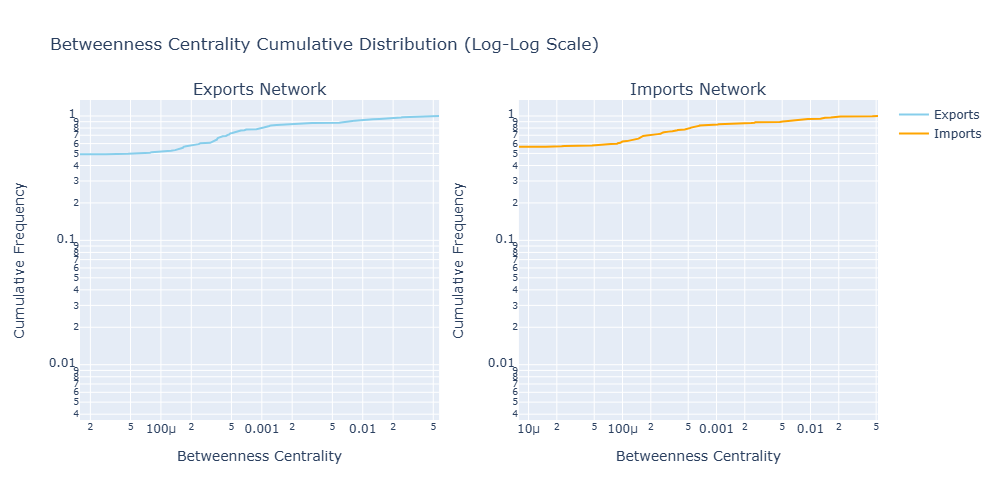
\includegraphics[scale=0.4]{img/betweencum.png}
\label{fig:betweencum}
\end{figure}
The networks are again dominated by a few central countries with high betweenness centrality, which are crucial for maintaining the network's connectivity and facilitating trade flows. Most countries are on the periphery with low betweenness centrality, indicating they play minor roles in connecting other countries.

The sharp increase in the cumulative frequency at low centrality values followed by a long tail confirm the typical power-law distribution.
\subsubsection{Closeness Centrality}

\begin{figure}[ht]
\centering
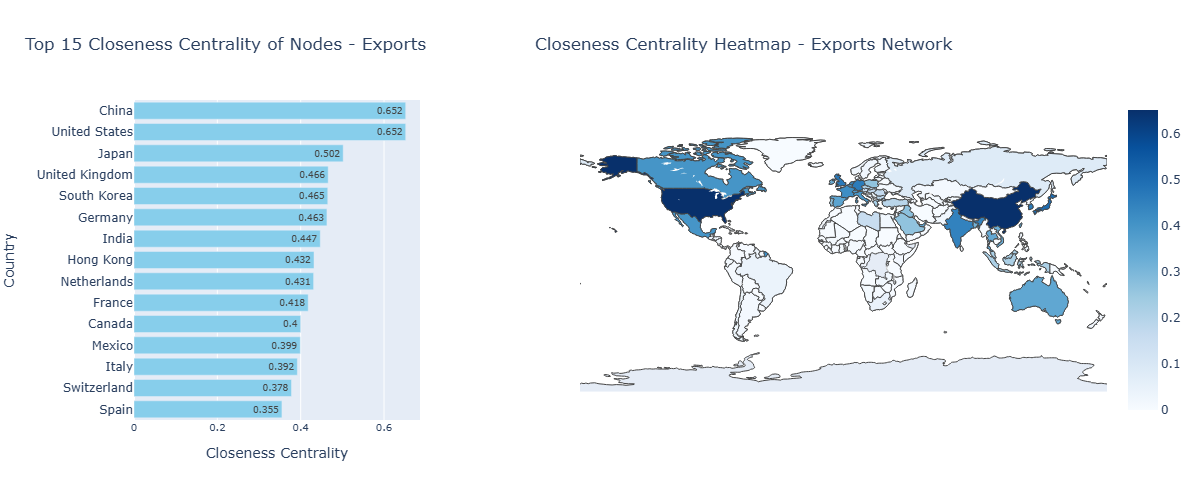
\includegraphics[width=\textwidth]{img/exportclose.png}
\label{fig:exportclose}
\end{figure}
China holds the top spot in both the import and export networks, showing its pivotal role in international trade. Due to its vast trade links, as evidenced by its high closeness centrality values, it is an important hub for both import and export. Although its closeness centrality is larger in the exports network, the US is ranked highly in both networks. This implies that although the US plays a major role in both importing and exporting, its exporting function is marginally more prominent in terms of connectivity. With their vast trade links, China and the US are important hubs in the global commerce network that are essential for both importing and exporting. Their prominence places them in a crucial role for maintaining the stability of the world economy.

Germany shines out in both the exports network and the imports network, although nations like the United Kingdom, France, and the Netherlands are more prevalent. This suggests that a number of European countries have a significant export focus.

Due to the region's rapid economic expansion and industrialization, Asia has seen a substantial shift in the dynamics of global trade, as seen by the high centrality scores of some Asian nations.

\begin{figure}[ht]
\centering
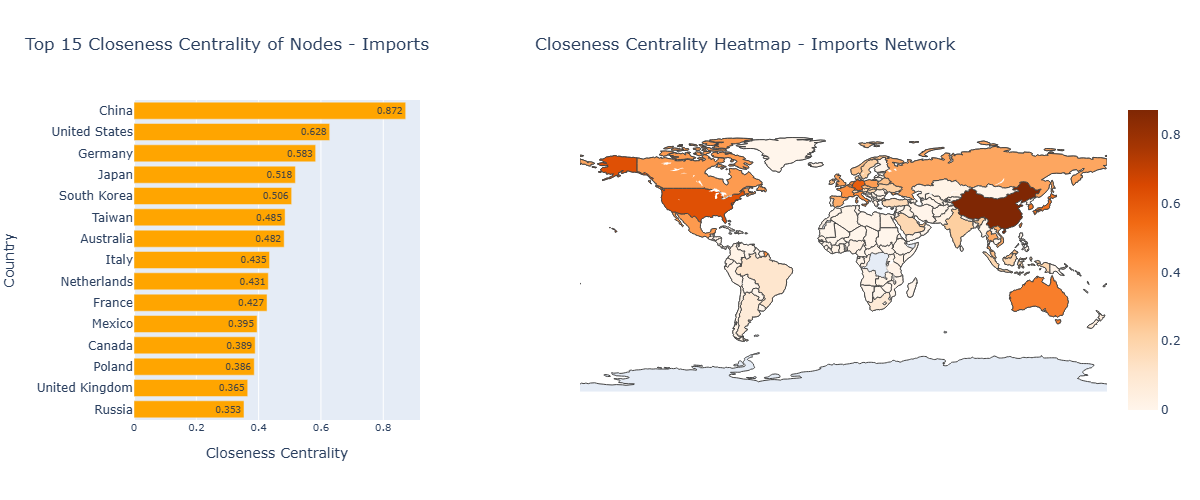
\includegraphics[width=\textwidth]{img/importclose.png}
\label{fig:importclose}
\end{figure}
\subsubsection{Pagerank}
\begin{figure}[ht]
\centering
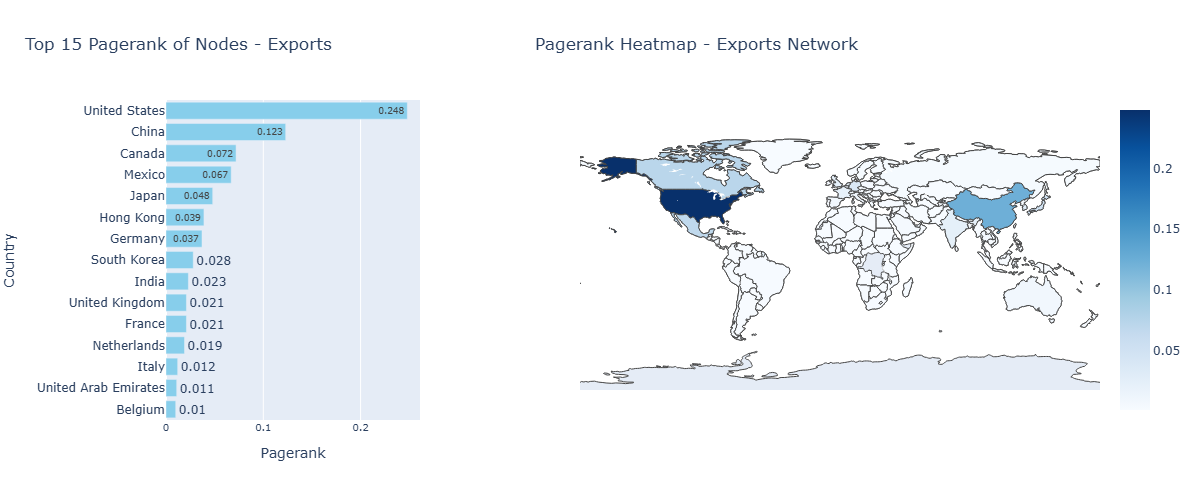
\includegraphics[width=\textwidth]{img/exportpr.png}
\label{fig:exportpr}
\end{figure}
Central economic hubs are those nations with the greatest PageRank values, such as China and the United States. Their significant contributions to imports and exports demonstrate their extensive trading networks and economic clout. High PageRank values in both exports and imports indicate nations with robust, mutually beneficial trade ties. For instance, due to their interconnected supply chains and reciprocal trade dependence, China and the United States are both significant exporters and importers.
Countries with high PageRank values within specific regions indicate regional economic leaders. For instance, Germany and the Netherlands are significant in Europe, while South Korea and Japan are prominent in Asia. Countries that appear in the top ranks for both exports and imports, like Germany, Japan, and South Korea, demonstrate diversified economies with significant import needs to support their exports.
Brazil and India are examples of rising economies with moderate PageRank values that are becoming more significant players in international trade. Their increasing integration into global trade networks reflects economic growth and diversification.


\begin{figure}[ht]
\centering
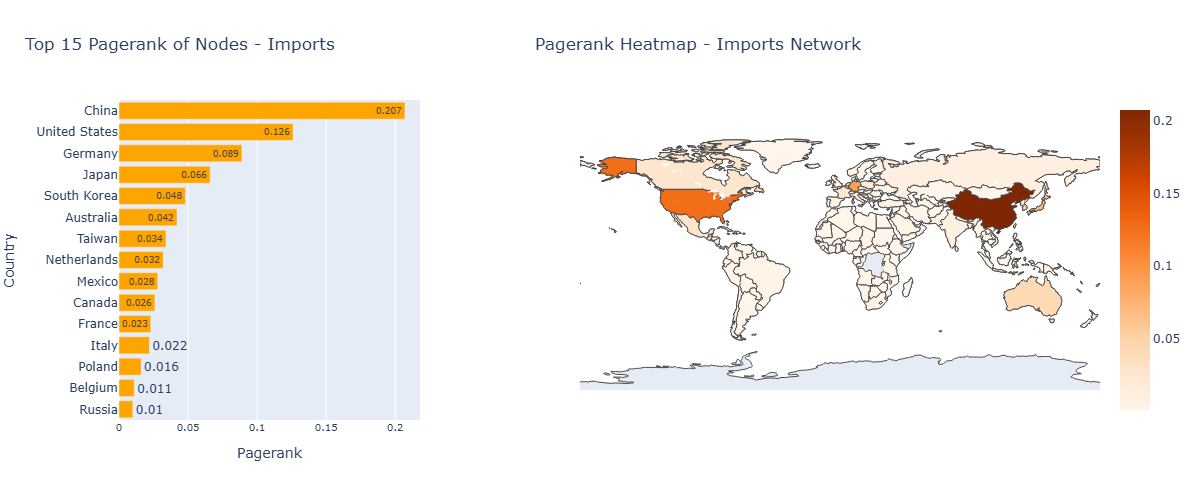
\includegraphics[width=\textwidth]{img/importpr.png}
\label{fig:importpr}
\end{figure}

\subsubsection{Local Clustering Coefficient}
\begin{figure}[ht]
\centering
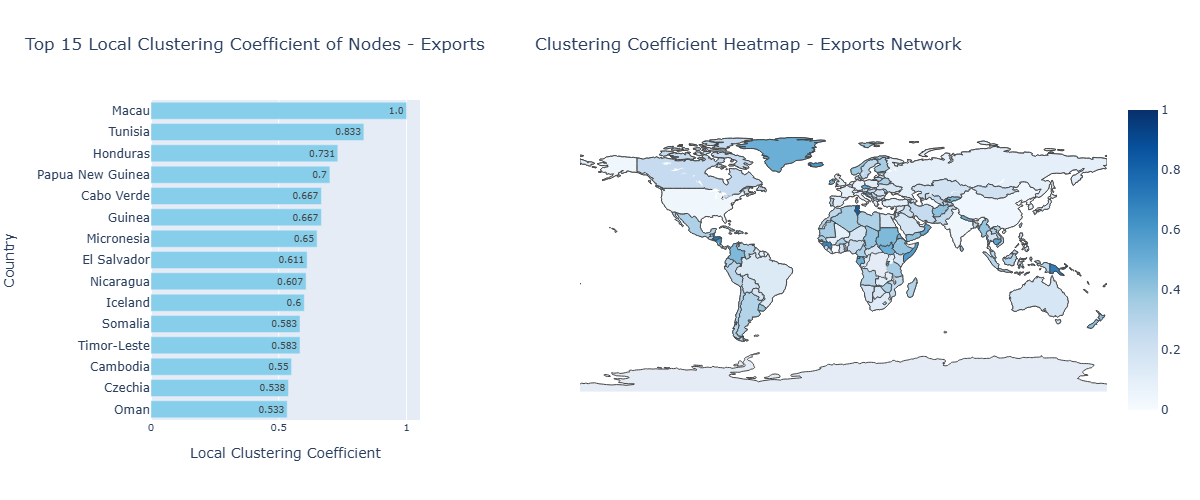
\includegraphics[width=\textwidth]{img/exportlcc.png}
\label{fig:exportlcc}
\end{figure}
Macau (1.0000): Because of its status as a free port and regional hub in Asia, total clustering suggests that Macau's trading partners are completely integrated.

Tunisia (0.8333): The country's high clustering indicates robust regional trade in the Mediterranean and North Africa.

The significant clustering of Honduras (0.7308), El Salvador (0.6111), and Nicaragua (0.6071) in Central America is indicative of the impact of regional trade agreements such as CAFTA-DR.

Micronesia (0.6500), and Papua New Guinea (0.7000): High clustering suggests robust regional trade within the Pacific Islands.

Czechia (0.5385), Croatia (0.4808), Luxembourg (0.4667), and Slovenia (0.4630): These countries demonstrate how integrated the internal market of the European Union is.

\begin{figure}[ht]
\centering
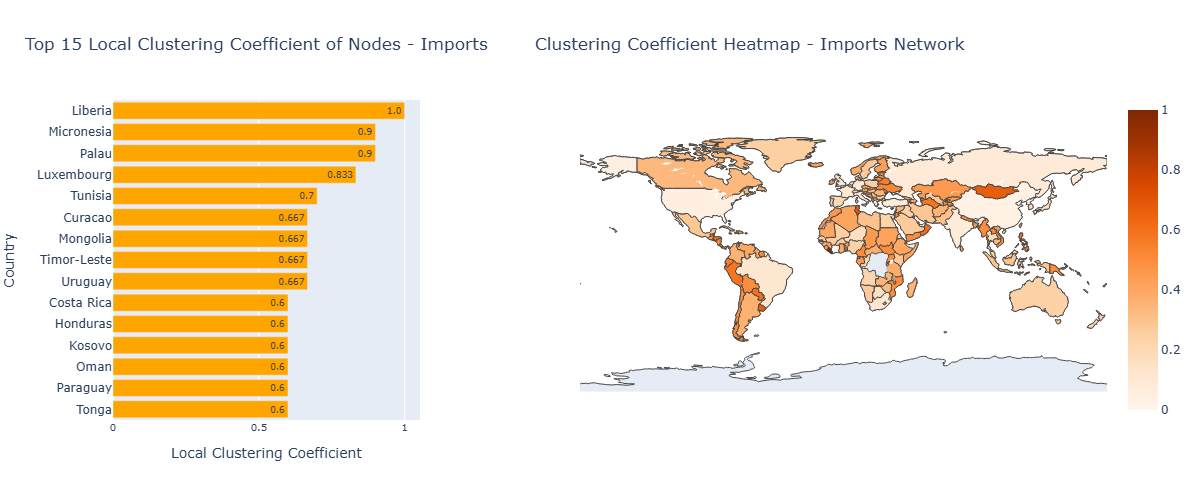
\includegraphics[width=\textwidth]{img/importlcc.png}
\label{fig:importlcc}
\end{figure}
Liberia (1.0000): Because of its strategic importance as a hub for maritime registry, full clustering indicates that the country's trading partners are all linked.

Micronesia (0.9000) and Palau (0.9000): Demonstrate robust intra-Pacific commerce.

Luxembourg (0.8333): Shows its pivotal position in the European economy by virtue of its intricately linked trading relationships.

Curacao (0.6667) and Tunisia (0.7000): Strong regional trade links in North Africa and the Caribbean can be observed by their high clustering.

High clustering implies active participation in regional trade networks throughout South America (Uruguay, 0.6667), and Central America (Costa Rica, 0.6000).

Oman (0.6000), Qatar (0.4333): Shows how trade within the Gulf Cooperation Council (GCC) is interrelated.
\subsubsection{Correlation between Local Clustering Coefficient and Degree Centrality}
\begin{figure}[ht]
\centering
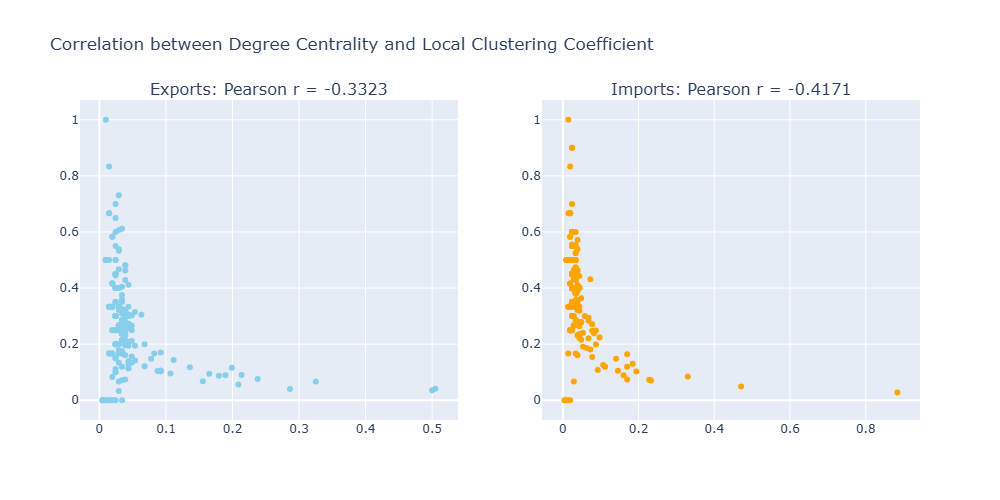
\includegraphics[width=\textwidth]{img/correlation.png}
\label{fig:importlcc}
\end{figure}
Both networks show a negative correlation between LCC and DC. This suggests that as the number of trade connections (degree centrality) increases, the interconnectedness among those connections (local clustering coefficient) tends to decrease. The imports network has a stronger negative correlation (-0.4171) compared to the exports network (-0.3323). This indicates that the tendency for a decrease in clustering with increasing trade connections is more pronounced in the imports network.

Distribution Patterns:

Exports Network: -High LCC, Low DC: Many countries have a few but highly interconnected trade partners. -Low LCC, High DC: Countries with many trade partners tend to have these partners less interconnected.

Imports Network: Similar pattern to the exports network but with a more pronounced negative correlation.

In both networks, there are outliers with LCC close to 1.0 but with very low DC, indicating countries with perfect clustering but minimal trade connections.

In both exports and imports networks, countries with high DC but low LCC can be considered trade hubs while countries with high LCC and low DC are likely part of more specialized and localized trade networks. The observed patterns suggest that countries engage in diversified trade (high DC) at the expense of interconnected trade networks (high LCC).
\subsubsection{Cliques}
\subsubsection{K-cores Decomposition}
\subsubsection{Assortative Mixing by Degree}
\begin{itemize}
\item \textbf{Exports Network}: -0.0221
\item \textbf{Imports Network}: -0.1176
\end{itemize}
The exports network shows a slight negative assortative mixing by degree: countries with different degrees of exporting activities (degree referring to the number of export relationships) tend to trade with each other more often than those with similar export capacities. This suggests that in the exports network, countries with diverse export capacities engage in trade relationships. Countries exporting a wide range of goods might seek to balance their trade portfolio by engaging with partners that have complementary rather than similar export profiles.

The imports network exhibits a more pronounced negative assortative mixing by degree compared to the exports network. Countries with different degrees of importing activities (number of import relationships) tend to be more connected than those with similar import capacities. In the imports network, countries importing a variety of goods might prefer to source from partners with diverse export capabilities. This behavior can support strategic sourcing strategies where countries aim to mitigate risks by diversifying import sources.

The imports network exhibits a stronger negative assortative mixing compared to the exports network (-0.1176 vs -0.0221): diversity in import partners may be more strategically valued than in export relationships.
\subsubsection{Density}
\begin{itemize}
\item \textbf{Exports Network}: 0.0228
\item \textbf{Imports Network}: 0.0235
\end{itemize}
Exports Network: Graph Density (0.0228): approximately 2.28\% of all possible export relationships between countries actually exist in the network. The low graph density suggests that the exports network is sparse, meaning that not all potential trade relationships are currently realized.

The imports network shows a slightly higher graph density of 0.0235. Similar to the exports network, the imports network is also relatively sparse. There is potential for increasing the number of import relationships to diversify sources and mitigate risks associated with dependency on specific countries or regions.

The low graph densities observed in both exports and imports networks suggest opportunities for enhancing connectivity and expanding trade relationships among countries. Policymakers and stakeholders can leverage these insights to foster a more resilient and interconnected global trade environment, thereby promoting economic growth and stability on an international scale.
\section{Conclusion}
\label{conclusion}

The study's quantitative findings reveal significant insights into the structure of international trade. Key players identified through centrality measures are crucial for understanding global trade dynamics. The analysis highlights the importance of certain countries as major hubs, which can influence economic stability and policy making. These findings underscore the value of network analysis in economic studies.

\section{Critique}
\label{critique}

The work addresses the problem of understanding international trade networks to a significant extent by identifying key players and patterns. However, there are areas for improvement:

Data Quality: Gathering more detailed and up-to-date trade data could enhance the accuracy of the analysis.
Model Complexity: Incorporating additional factors such as trade volumes and economic indicators could provide a more comprehensive view.
Alternative Measures: Exploring other network measures or machine learning approaches could yield further insights.
Overall, the study provides a solid foundation for understanding international trade networks but could benefit from deeper and more nuanced analysis.

\end{document}